\section{Поставить собственную ЭЦП на файл}

Для того, чтобы начать работать с gpg, сначала необходимо сгенерировать собственную пару ключей, состоящую из публичной (сертификат)
и приватной частей. Публичный ключ может распространяться свободно (в том числе и в сети Интернет), в то время как передача
приватного ключа третьим лицам категорически запрещена. Для того, чтобы сгенерировать пару ключей с помощью  gpg необходимо 
воспользоваться опцией \src{--gen-key}. Пример вывода утилиты gpg при использовании данной опции представлен ниже в листинге 
\ref{lst:gen-key}. 
\\ \hfill \\
\inputminted[lastline=23]{console}{resources/01_gen_key}
\inputminted[firstline=25]{console}{resources/01_gen_key}
\captionof{listing}{Вывод утилиты gpg при вызове с опцией \src{--gen-key} \label{lst:gen-key}}

\begin{figure}[H]
    \centering
    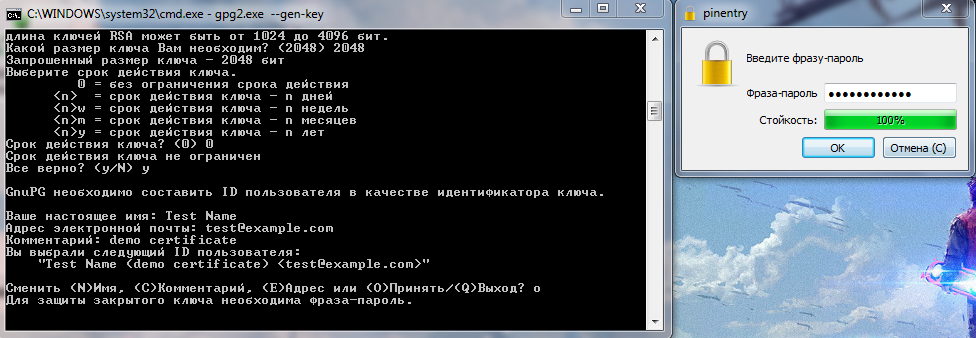
\includegraphics[width=16cm]{resources/02_gen_key.png}
    \caption{Форма ввода пароля при генерации ключей в gpg}
    \label{fig:gen-key-password-form}
\end{figure}

При этом в строке $34$ вывода происходит предоставление пользователю формы для ввода пароля генерируемого приватного ключа. В случаях,
когда приватный ключ скомпрометирован, данный пароль является последней ступенью защиты перед злоумышленниками. Форма ввода пароля
показана на рисунке \ref{fig:gen-key-password-form}. После ее ввода требуется также подтверждение выбранного пароля.

Для дальнейшего использования созданных ключей необходимо сначала экспортировать свой сертификат для того, чтобы его можно было 
передать лицам, заинтересованным в отправке зашифрованных и/или подписанных сообщений пользователю. Для этого необходимо 
воспользоваться опцией \src{--export}. Дополнительно также можно использовать опции \src{--armor}, которая преобразовывает вывод из 
бинарного формата в формат ASCII, и \src{--output} для указания файла записи результата. Пример вызова утилиты gpg с опцией 
\src{--export} представлен в листинге \ref{lst:export-certificate}.

\begin{listing}[H]
    \inputminted[lastline=14]{console}{resources/03_export_certificate}
    \caption{Вывод утилиты gpg при вызове с опцииями \src{--export} и \src{--armor}}
    \label{lst:export-certificate}
\end{listing}

Одним из основных сценариев использования утилиты gpg --- это установка электронной цифровой подписи. Для установки ЭЦП на какой-либо
файл необходимо воспользоваться опцией \src{--sign} или \src{--detach-sign} как показано в листинге \ref{lst:sign-file}.

\begin{listing}[H]
    \inputminted{console}{resources/04_sign_file}
    \caption{Вывод утилиты gpg при вызове с опцией \src{--detach-sign}}
    \label{lst:sign-file}
\end{listing}

После выполнения этой команды будет создан отдельный файл цифровой подписи. Его содержание представлено в листинге \ref{lst:file-sign}

\begin{listing}[H]
    \inputminted{console}{resources/05_file_sign}
    \caption{Пример цифровой подписи}
    \label{lst:file-sign}
\end{listing}